\section{Problem analysis}

The host organization, Khonraad Software Engineering, a subsidiary of Visma, provides mission-critical services focussed on the automation of workflows at the cross-section of local government and healthcare.
Specifically, Khonraad facilitates the mental health care and coercion laws in the Netherlands - WVGGZ, WZD, and WTH - which provide agencies the ability to intervene in domestic violence, psychiatric disorders, and illnesses.

Khonraad's system facilitates reporting and communication between municipalities, police, judiciary, lawyers, mental health care, and many social care institutions.
The system has 15,000 users and is available 24/7. 

Configuration and administration use complex matrices of compliance mechanisms, access user rights and communication settings.
The sensitivity of the personal data, being both medical and criminal, means security is of utmost importance.
The security against data loss, preventing unlawful disclosure and guaranteeing availability, especially during crisis situations, are crucial.
Demonstration of the correctness of the, often changing, configuration is a major concern in the company. 

This configuration is done in a business rule system. 
A business rules engine executes rules at runtime. 
``Rules specify conditions to be monitored and operations that should be executed when certain conditions are detected.
Rather than continuously monitoring the simulation, experts can define and deploy appropriate rules that are automatically evaluated at runtime''\cite{liu2003dios++}. 

Specifically, the rules engine used is JBoss Rules, more commonly known as Drools, from JBoss, a subsidiary of RedHat\cite{browne2009jboss}.
Drools is a framework for Rule-Based development.
It is an open-source production rule system for complex event processing, using the ReteOO and Phreak implementations of the pattern matching Rete algorithm\cite{forgy1989rete}.
The rules are described in a Domain Specific Language (DSL).
These are stored in Drools (.drl) files. 
An example of a DRL file can be seen in figure \ref{fig:drl_file}. 

\begin{figure}[h]
    \centering
    \fbox{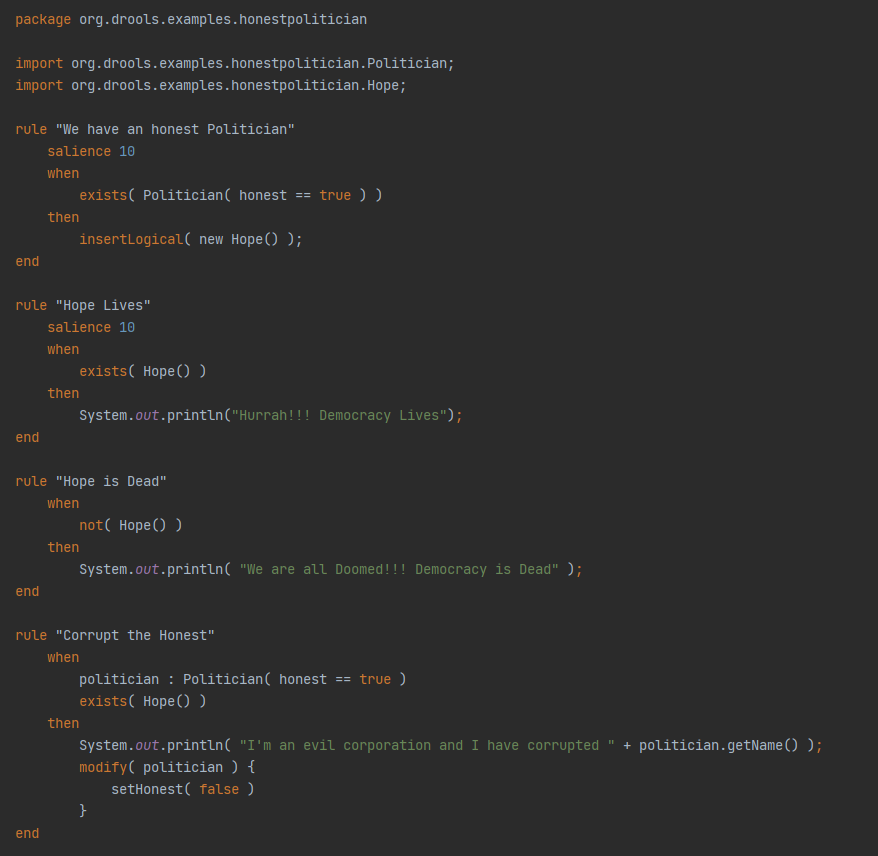
\includegraphics[width=0.80\textwidth]{images/droolsExample.png}}
    \caption{Example drools file}
    \label{fig:drl_file}
\end{figure}

Reasoning over a small number of rules is already surprisingly hard.
Our host organization has many rules and, thus, reasoning about them is particularly challenging.

The Drools language does not have tooling in standard IDEs to help developers to reason about the code.
The problem of a lack of useful visualization for Drools has been known as far back as 2011, when Kaczor, et al\cite{kaczor2011visual} proposed a method of visualising Drools. 
There have also been a few commercial tools to help.
However, these all suffer from the fact that they are not integrated and thus have parsing issues and a lack of immediate feedback. 

We have observed the difficulty that developers have trying to reason about and edit collections of Drools files.
We hypothesize that developers can be presented with different views on their code that will allow them to better understand the code.
The problem we wish to solve - how to improve the ability to reason about large collections of Drools rules - we believe, lends itself to the technique of projectional editing.

Editing programs in a text editor means that you must match the syntax for the parsers to transform the text into an AST.
Projectional editors are editors in which a user edits the abstract syntax tree directly without using a parser\cite{voelter2014generic}.
This potentially allows for almost unlimited language composition and flexible notations.
Like MVC Pattern, changes in one projection of the AST will instantly be visible and editable in another projection\cite{guttormsen2017consistent}.

By using projections to improve feedback whilst coding, we believe that this can reduce the representation impedance mismatch that hampers developer's reasoning.
To build a projectional language in the time available for this project we would need a viable language workbench.
